% Copyright 2004 by Till Tantau <tantau@users.sourceforge.net>.
%
% In principle, this file can be redistributed and/or modified under
% the terms of the GNU Public License, version 2.
%
% However, this file is supposed to be a template to be modified
% for your own needs. For this reason, if you use this file as a
% template and not specifically distribute it as part of a another
% package/program, I grant the extra permission to freely copy and
% modify this file as you see fit and even to delete this copyright
% notice. 

\documentclass{beamer}
\usepackage{graphics} % for pdf, bitmapped graphics files
\usepackage{graphicx}
\usepackage{verbatim} 
%\usepackage{pstricks}
%\usepackage{epstopdf}
% Generated with LaTeXDraw 2.0.8
% Wed Feb 18 16:25:36 IST 2015
\usepackage{amsmath} % assumes amsmath package installed
%\usepackage{amssymb}  % assumes amsmath package installed
\usepackage{algorithm} % assumes amsmath package installed
\usepackage{algpseudocode}
\usepackage{subfigure}
\usepackage{multirow}
\usepackage{algpseudocode}
\usepackage[pdf]{pstricks}
\usepackage{epsfig}
\usepackage{pst-grad} % For gradients
\usepackage{pst-plot} % For axes
\usepackage{epsfig} % for post
% There are many different themes available for Beamer. A comprehensive
% list with examples is given here:
% http://deic.uab.es/~iblanes/beamer_gallery/index_by_theme.html
% You can uncomment the themes below if you would like to use a different
% one:
%\usetheme{AnnArbor}
%\usetheme{Antibes}
%\usetheme{Bergen}
%\usetheme{Berkeley}
%\usetheme{Berlin}
%\usetheme{Boadilla}
\usetheme{boxes}
%\usetheme{CambridgeUS}
%\usetheme{Copenhagen}
%\usetheme{Darmstadt}
%\usetheme{default}
%\usetheme{Frankfurt}
%\usetheme{Goettingen}
%\usetheme{Hannover}
%\usetheme{Ilmenau}
%\usetheme{JuanLesPins}
%\usetheme{Luebeck}
%\usetheme{Madrid}
%\usetheme{Malmoe}
%\usetheme{Marburg}
%\usetheme{Montpellier}
%\usetheme{PaloAlto}
%\usetheme{Pittsburgh}
%\usetheme{Rochester}
%\usetheme{Singapore}
%\usetheme{Szeged}
%\usetheme{Warsaw}

\title{Mobile Robot Navigation Amidst Humans with Intents and Uncertainties:A Time Scaled Collision cone Approach}

% A subtitle is optional and this may be deleted
\subtitle{}

\author{Akhil Nagariya\inst{1} \and Bharath Gopalakrishna\inst{1} \and Arun Singh\inst{2} \and Krishnam Gupta \inst{1} \and K Madhava Krishna \inst{1}}
% - Give the names in the same order as the appear in the paper.
% - Use the \inst{?} command only if the authors have different
%   affiliation.

\institute[Universities of Somewhere and Elsewhere] % (optional, but mostly needed)
{
  \inst{1}%
  RRC\\
  IIIT Hyderabad
  \and
  \inst{2}%
  Ben-Gurion University, Isreal
  }
% - Use the \inst command only if there are several affiliations.
% - Keep it simple, no one is interested in your street address.

\date{CDC 2015}
% - Either use conference name or its abbreviation.
% - Not really informative to the audience, more for people (including
%   yourself) who are reading the slides online

\subject{Theoretical Computer Science}
% This is only inserted into the PDF information catalog. Can be left
% out. 

% If you have a file called "university-logo-filename.xxx", where xxx
% is a graphic format that can be processed by latex or pdflatex,
% resp., then you can add a logo as follows:

% \pgfdeclareimage[height=0.5cm]{university-logo}{university-logo-filename}
% \logo{\pgfuseimage{university-logo}}

% Delete this, if you do not want the table of contents to pop up at
% the beginning of each subsection:
\AtBeginSubsection[]
{
  \begin{frame}<beamer>{Outline}
    \tableofcontents[currentsection,currentsubsection]
  \end{frame}
}

% Let's get started
\begin{document}

\begin{frame}
  \titlepage
\end{frame}

\begin{frame}{Outline}
  \tableofcontents
  % You might wish to add the option [pausesections]
\end{frame}

% Section and subsections will appear in the presentation overview
% and table of contents.
\section{Motivation}


\subsection{}

\begin{frame}{Motivation}
  \begin{itemize}
  \item {
   Robots and humans are beginning to occupy the same work spaces
  }
  \item {
   Account for human intent in robot's navigation and avoidance Maneuver
  }
  \item {
    Uncertain and Haphazard local movements of human 
  }
  \end{itemize}
\end{frame}


%\subsection{Second Subsection}

% You can reveal the parts of a slide one at a time
% with the \pause command:
%\begin{frame}{Second Slide Title}
 % \begin{itemize}
 % \item {
  %  First item.
   % \pause % The slide will pause after showing the first item
 % }
 % \item {   
  %  Second item.
  %}
  % You can also specify when the content should appear
  % by using <n->:
  %\item<3-> {
   % Third item.
  %}
  %\item<4-> {
   % Fourth item.
  %}
  % or you can use the \uncover command to reveal general
  % content (not just \items):
  %\item<5-> {
   % Fifth item. \uncover<6->{Extra text in the fifth item.}
  %}
  %\end{itemize}
%\end{frame}

\section{Human Intention prediction}

\subsection{•}

\begin{frame}{Human Intention prediction}
%\begin{block}{Block Title}
%You can also highlight sections of your presentation in a block, with it's own title
%\end{block}
%\begin{theorem}
%There are separate environments for theorems, examples, definitions and proofs.
%\end{theorem}
%\begin{example}
%Here is an example of an example block.
%\end{example}
\begin{itemize}
\item{Characterize intents as the final destinations a person might reach}
\item{Let $D = \{\mathbf{d^1,d^2,...,d^m}\}$ be the set of final destinations a person can go to in a given environment}
\item{compute the probability of each of these intents Using Hidden Markov Model.}
\item{Characterize local Haphazard movements as a gaussian $\mathcal{N}(\mu_i(\mathbf{x}^{t}),\sigma_t)$ }
\end{itemize}
\end{frame}
\begin{frame}{Human Intention prediction}
\begin{figure}
\centering
\includegraphics[width= 8.1cm, height=4.5cm]{screen1.eps}
\end{figure}
\end{frame}
\begin{frame}{HMM for Intention prediction}
\begin{itemize}
\item{ Let $S^t \in D$ represent the intent of a person to reach destination $S^t$ at time $t$.}
\item{$D$ represents set of states in HMM.}
\item{Human trajectories are represented as $X(T) = \{\mathbf{x^1,x^2,...,x^T}\}$}
\end{itemize}

\end{frame}
\begin{frame}{HMM for Intention prediction}
\begin{itemize}
\item{  $O^t$ is the angle defined by the first derivative of the trajectory at point $\mathbf{x^t}$}
\item{Given the current position and orientation we compute the probability of reaching each of the destination $d^i \in D$}

\end{itemize}
\begin{figure}[thpb]
 \scalebox{1} % Change this value to rescale the drawing.
{
\begin{pspicture}(0,-3.636)(9.053437,3.665)
\definecolor{color10022}{rgb}{0.9803921568627451,0.10196078431372549,0.1450980392156863}
\definecolor{color10027}{rgb}{0.12549019607843137,0.19215686274509805,0.8470588235294118}
\definecolor{color10030}{rgb}{0.09803921568627451,0.9372549019607843,0.26666666666666666}
\definecolor{color10042}{rgb}{0.043137254901960784,0.9411764705882353,0.9411764705882353}
\definecolor{color10038}{rgb}{0.07450980392156863,0.1568627450980392,0.9568627450980393}
\definecolor{color2}{rgb}{0.13333333333333333,0.21176470588235294,0.9411764705882353}
\definecolor{color3}{rgb}{0.09411764705882353,0.2196078431372549,0.9450980392156862}
\definecolor{color10046}{rgb}{0.2,0.23921568627450981,0.9529411764705882}
\definecolor{color5}{rgb}{0.08627450980392157,0.9176470588235294,0.9490196078431372}
\psbezier[linewidth=0.022,linecolor=color10022](0.28,-3.625)(0.0,-1.925)(2.712876,0.108493745)(3.64,0.555)(4.567124,1.0015062)(4.74,0.915)(5.4,0.875)
\psdots[dotsize=0.12](2.38,2.635)
\psdots[dotsize=0.12](5.3,3.375)
\psline[linewidth=0.04,linecolor=color10027,arrowsize=0.05291667cm 2.0,arrowlength=1.4,arrowinset=0.4]{<-}(2.38,2.595)(3.18,0.315)(5.26,3.335)
\psline[linewidth=0.04cm,linecolor=color10030,arrowsize=0.05291667cm 2.0,arrowlength=1.4,arrowinset=0.4]{->}(1.36,-0.845)(5.44,1.755)
\psline[linewidth=0.04cm,linestyle=dashed,dash=0.16cm 0.16cm,arrowsize=0.05291667cm 2.0,arrowlength=1.4,arrowinset=0.4]{->}(3.22,0.295)(8.6,0.355)
\usefont{T1}{ptm}{m}{n}
\rput(1.9990625,2.62){\color{color2}\psframebox*[framesep=0, boxsep=false,fillcolor=white] {$d_j$}}
\usefont{T1}{ptm}{m}{n}
\rput(5.7096877,3.48){\color{color3}$d_i$}
\psarc[linewidth=0.012,linecolor=color10038,arrowsize=0.05291667cm 2.0,arrowlength=1.4,arrowinset=0.4]{->}(3.84,0.515){0.46}{-35.247574}{113.19859}
\psarc[linewidth=0.025999999,linecolor=color10030,arrowsize=0.05291667cm 2.0,arrowlength=1.4,arrowinset=0.4]{->}(4.5,0.735){0.64}{-45.0}{69.443954}
\psarc[linewidth=0.022,linecolor=color10046,arrowsize=0.05291667cm 2.0,arrowlength=1.4,arrowinset=0.4]{->}(3.47,0.485){1.31}{61.88679}{124.69515}
\usefont{T1}{ptm}{m}{n}
\rput(3.3323438,1.4){$\theta_{i,j}(t)$}
\usefont{T1}{ptm}{m}{n}
\rput(4.833906,0.62){\color{color10030}$O^t$}
\usefont{T1}{ptm}{m}{n}
\rput(3.8723438,0.46){$u_i(t)$}
\psline[linewidth=0.03cm,linestyle=dashed,dash=0.16cm 0.16cm,arrowsize=0.05291667cm 2.0,arrowlength=1.4,arrowinset=0.4]{<-}(0.48,-2.645)(1.78,-2.125)
\usefont{T1}{ptm}{m}{n}
\rput(2.6571875,-2.08){trajecjtory}
\psline[linewidth=0.016cm,linestyle=dashed,dash=0.16cm 0.16cm,arrowsize=0.05291667cm 2.0,arrowlength=1.4,arrowinset=0.4]{<-}(5.06,0.675)(6.74,1.235)
\usefont{T1}{ptm}{m}{n}
\rput(7.890625,1.36){\color{color10030}current heading}
\psdots[dotsize=0.12](3.22,0.335)
\psline[linewidth=0.016cm,linestyle=dashed,dash=0.16cm 0.16cm,arrowsize=0.05291667cm 2.0,arrowlength=1.4,arrowinset=0.4]{<-}(3.22,0.335)(3.7,-0.865)
\usefont{T1}{ptm}{m}{n}
\rput(3.7279687,-0.88){xt}
%\rput(7.5671873,3.52){Realtive \\ measure between $d_i$ and $d_j$ \\ with respect to $x^t$}
\usefont{T1}{ptm}{m}{n}
\rput(7.2614064,0.08){x-axis}
%\psline[linewidth=0.016cm,linestyle=dashed,dash=0.16cm 0.16cm,arrowsize=0.05291667cm 2.0,arrowlength=1.4,arrowinset=0.4]{<-}(3.54,1.795)(3.74,3.415)
\end{pspicture} 
}
\caption{figure shows the heading angle $O^t$, $\mu_{ij}(t)$ and $\mu_{i}(t)$ at time $t$}
\label{notation}
\end{figure}
\end{frame}
\begin{frame}{HMM for Intention prediction}
\begin{itemize}
\item{  $\mu_i(t)$ is the measure relative to the destination $\mathbf{d^i}$}
\item{$O^t$ is the global measure of the target orientation}
\item{$\theta_{ij}(t)$ is the measure between final destinations $\mathbf{d^i}$ and $\mathbf{d^j}$ relative to the current position $\mathbf{x^t}$}
\end{itemize}
\begin{figure}[thpb]
 \scalebox{1} % Change this value to rescale the drawing.
{
\begin{pspicture}(0,-3.636)(9.053437,3.665)
\definecolor{color10022}{rgb}{0.9803921568627451,0.10196078431372549,0.1450980392156863}
\definecolor{color10027}{rgb}{0.12549019607843137,0.19215686274509805,0.8470588235294118}
\definecolor{color10030}{rgb}{0.09803921568627451,0.9372549019607843,0.26666666666666666}
\definecolor{color10042}{rgb}{0.043137254901960784,0.9411764705882353,0.9411764705882353}
\definecolor{color10038}{rgb}{0.07450980392156863,0.1568627450980392,0.9568627450980393}
\definecolor{color2}{rgb}{0.13333333333333333,0.21176470588235294,0.9411764705882353}
\definecolor{color3}{rgb}{0.09411764705882353,0.2196078431372549,0.9450980392156862}
\definecolor{color10046}{rgb}{0.2,0.23921568627450981,0.9529411764705882}
\definecolor{color5}{rgb}{0.08627450980392157,0.9176470588235294,0.9490196078431372}
\psbezier[linewidth=0.022,linecolor=color10022](0.28,-3.625)(0.0,-1.925)(2.712876,0.108493745)(3.64,0.555)(4.567124,1.0015062)(4.74,0.915)(5.4,0.875)
\psdots[dotsize=0.12](2.38,2.635)
\psdots[dotsize=0.12](5.3,3.375)
\psline[linewidth=0.04,linecolor=color10027,arrowsize=0.05291667cm 2.0,arrowlength=1.4,arrowinset=0.4]{<-}(2.38,2.595)(3.18,0.315)(5.26,3.335)
\psline[linewidth=0.04cm,linecolor=color10030,arrowsize=0.05291667cm 2.0,arrowlength=1.4,arrowinset=0.4]{->}(1.36,-0.845)(5.44,1.755)
\psline[linewidth=0.04cm,linestyle=dashed,dash=0.16cm 0.16cm,arrowsize=0.05291667cm 2.0,arrowlength=1.4,arrowinset=0.4]{->}(3.22,0.295)(8.6,0.355)
\usefont{T1}{ptm}{m}{n}
\rput(1.9990625,2.62){\color{color2}\psframebox*[framesep=0, boxsep=false,fillcolor=white] {$d_j$}}
\usefont{T1}{ptm}{m}{n}
\rput(5.7096877,3.48){\color{color3}$d_i$}
\psarc[linewidth=0.012,linecolor=color10038,arrowsize=0.05291667cm 2.0,arrowlength=1.4,arrowinset=0.4]{->}(3.84,0.515){0.46}{-35.247574}{113.19859}
\psarc[linewidth=0.025999999,linecolor=color10030,arrowsize=0.05291667cm 2.0,arrowlength=1.4,arrowinset=0.4]{->}(4.5,0.735){0.64}{-45.0}{69.443954}
\psarc[linewidth=0.022,linecolor=color10046,arrowsize=0.05291667cm 2.0,arrowlength=1.4,arrowinset=0.4]{->}(3.47,0.485){1.31}{61.88679}{124.69515}
\usefont{T1}{ptm}{m}{n}
\rput(3.3323438,1.4){$\theta_{i,j}(t)$}
\usefont{T1}{ptm}{m}{n}
\rput(4.833906,0.62){\color{color10030}$O^t$}
\usefont{T1}{ptm}{m}{n}
\rput(3.8723438,0.46){$u_i(t)$}
\psline[linewidth=0.03cm,linestyle=dashed,dash=0.16cm 0.16cm,arrowsize=0.05291667cm 2.0,arrowlength=1.4,arrowinset=0.4]{<-}(0.48,-2.645)(1.78,-2.125)
\usefont{T1}{ptm}{m}{n}
\rput(2.6571875,-2.08){trajecjtory}
\psline[linewidth=0.016cm,linestyle=dashed,dash=0.16cm 0.16cm,arrowsize=0.05291667cm 2.0,arrowlength=1.4,arrowinset=0.4]{<-}(5.06,0.675)(6.74,1.235)
\usefont{T1}{ptm}{m}{n}
\rput(7.890625,1.36){\color{color10030}current heading}
\psdots[dotsize=0.12](3.22,0.335)
\psline[linewidth=0.016cm,linestyle=dashed,dash=0.16cm 0.16cm,arrowsize=0.05291667cm 2.0,arrowlength=1.4,arrowinset=0.4]{<-}(3.22,0.335)(3.7,-0.865)
\usefont{T1}{ptm}{m}{n}
\rput(3.7279687,-0.88){xt}
%\rput(7.5671873,3.52){Realtive \\ measure between $d_i$ and $d_j$ \\ with respect to $x^t$}
\usefont{T1}{ptm}{m}{n}
\rput(7.2614064,0.08){x-axis}
%\psline[linewidth=0.016cm,linestyle=dashed,dash=0.16cm 0.16cm,arrowsize=0.05291667cm 2.0,arrowlength=1.4,arrowinset=0.4]{<-}(3.54,1.795)(3.74,3.415)
\end{pspicture} 
}
\caption{figure shows the heading angle $O^t$, $\mu_{ij}(t)$ and $\mu_{i}(t)$ at time $t$}
\label{notation}
\end{figure}
\end{frame}
% Placing a * after \section means it will not show in the
% outline or table of contents.
\begin{frame}{HMM for Intention prediction}
\begin{itemize}
\item{$b_i(O^t)$ is the probability of observing heading $O^t$ given that the person is following the intent $\mathbf{d^i}$ at time $t$.}
$$
b_i(O^t) = p(O^t | S^t=\mathbf{d^i}) = \mathcal{N}(O^t | \mu_i(t),\sigma_o) 
$$ 
\item{$a_{ij}(t)$ is the probability that the human changes his intent from $\mathbf{d^i}$ to $\mathbf{d^j}$ at any discrete instant $t$ }
$$
a_{ij}(t) =p(S^{t+1}=\mathbf{d^j}|S^t = \mathbf{d^i})    = \eta \mathcal{N}(\theta_{ij}(t) | 0, \sigma_a) 
$$
\end{itemize}
\end{frame}
\begin{frame}{HMM for Intention prediction}
\begin{itemize}
\item{Let $O^{1:T}$ = $\{O^1,O^1,...,O^T\}$ is the set of measurements obtained till time $T$.}
\item{Our task is to calculate $p(S^t = \mathbf{d^i} | O^{1:T} 
,\lambda)$}

\item{ In HMM this term is usually referred to as $\gamma_t(i)$ To find this we use standard forward and backward algorithms.}
\end{itemize}

\end{frame}


\section{Proactive collision avoidance in intent space}
\subsection{}
\begin{frame}{Proactive collision avoidance in intent space}
\begin{itemize}
\item{To propose an optimization framework,
That achieves an elegant balance between minimizing risk and ease of collision avoidance maneuver.}
\item{Ease of Collision avoidance maneuver directly relates to factors like deviation from current path and acceleration and deceleration capabilities of robot.}
\item{Minimizing risk boils down to biasing the maneuver towards avoiding the most likely intent with higher confidence.}
\end{itemize}
\end{frame}
\begin{frame}{Proactive collision avoidance in intent space}
\begin{figure}
\centering
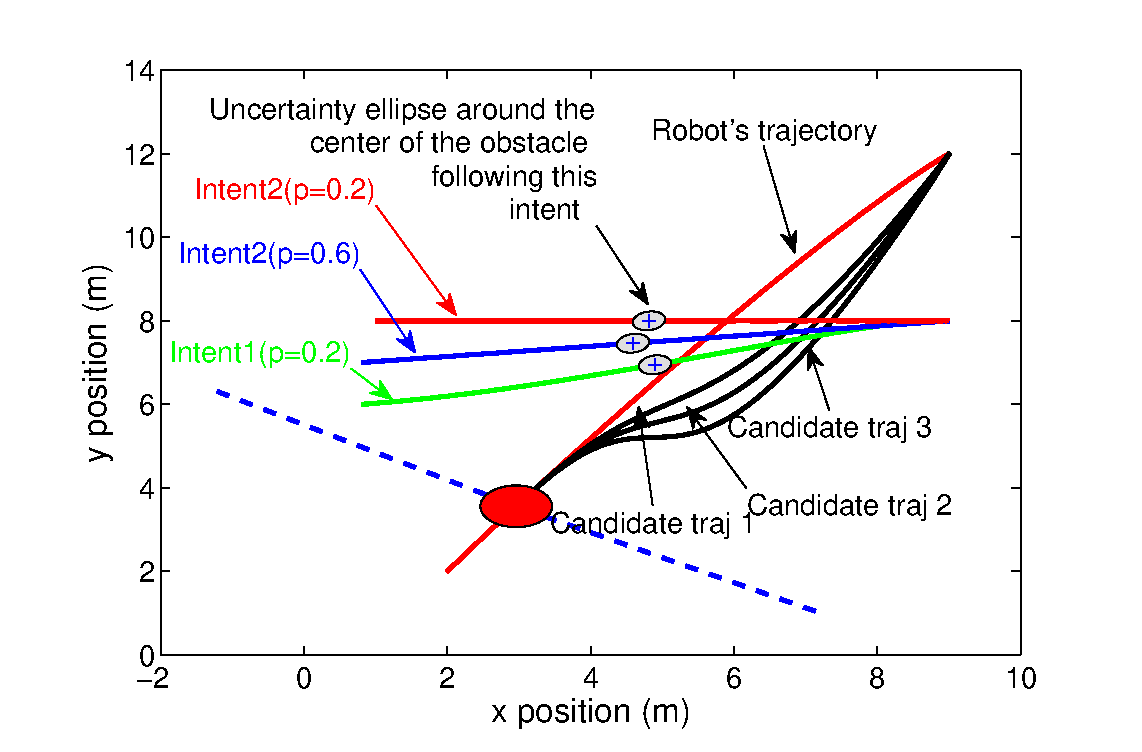
\includegraphics[width= 8.1cm, height=6.5cm]{full_plot.eps}
\end{figure}
\end{frame}
\begin{frame}{Proactive collision avoidance in intent space}
\begin{block}{Formulation steps}
\begin{itemize}
\item{Formulation for finding a relation between a particular collision avoidance maneuver and its confidence of safety, for a particular obstacle/intent.}
\end{itemize}
\begin{figure}
\centering
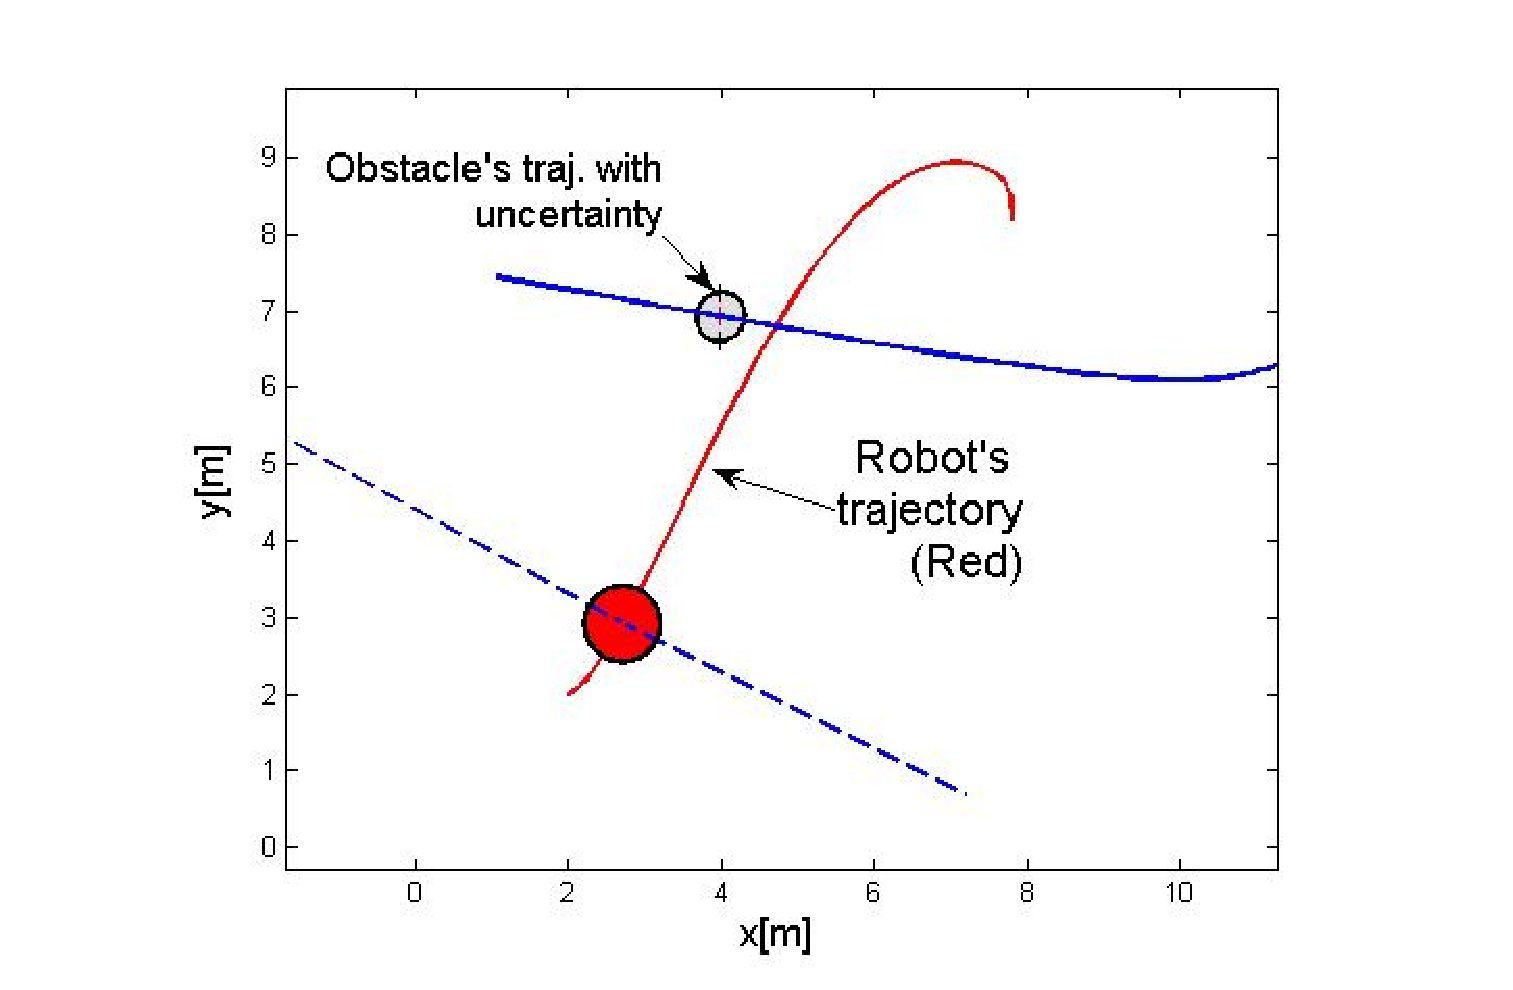
\includegraphics[width= 6.1cm, height=3.5cm]{fig1.eps}
\end{figure}
%You can also highlight sections of your presentation in a block, with it's own title
\end{block}
\end{frame}
\begin{frame}{Proactive collision avoidance in intent space}
\begin{block}{Formulation steps}
\begin{itemize}
\item{Formulation extending it to multiple                            intent space}
\end{itemize}
\begin{figure}
\centering
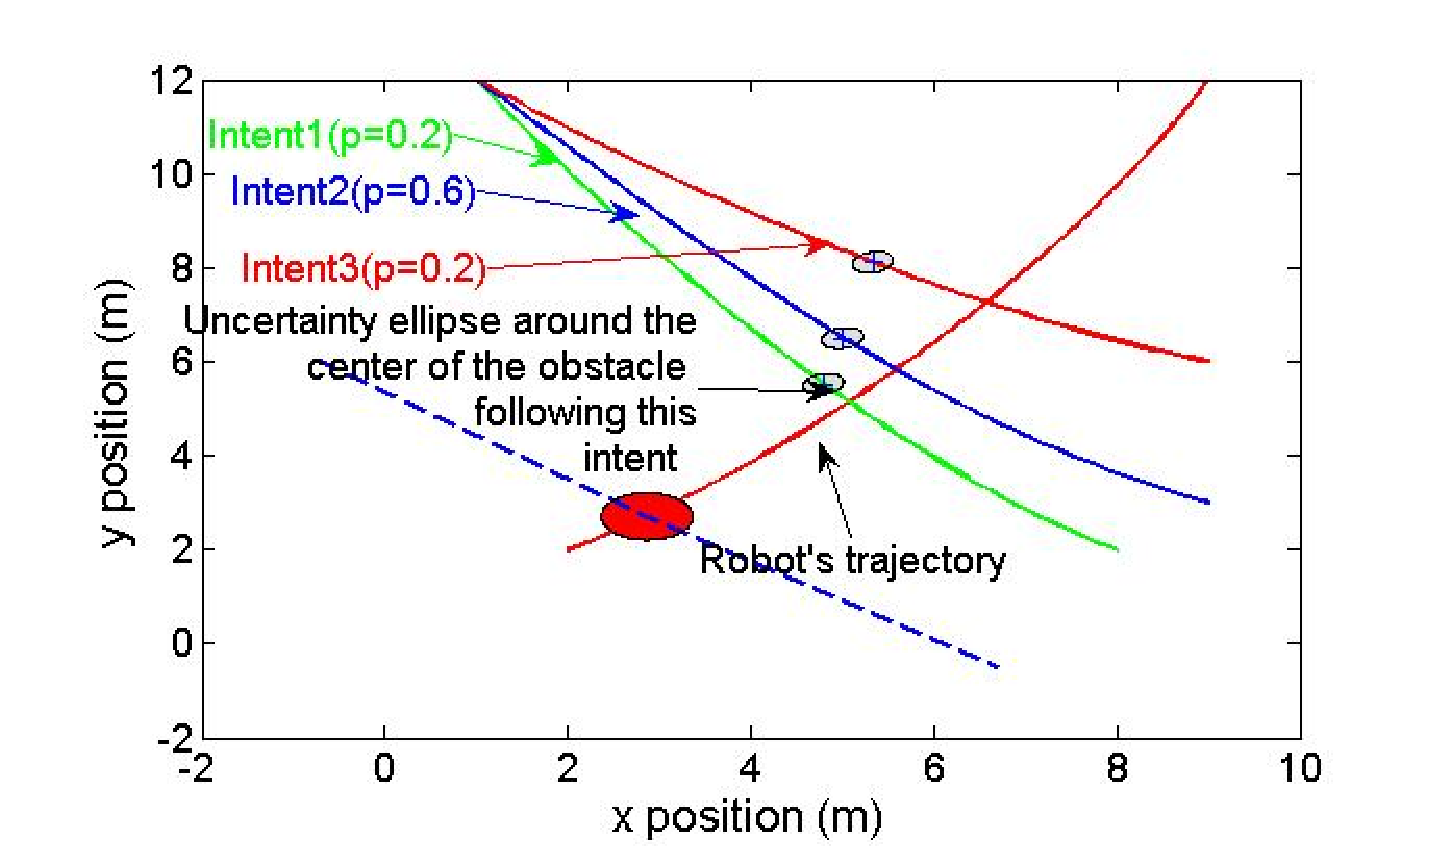
\includegraphics[width= 6.1cm, height=3.5cm]{fig2.eps}
\end{figure}
%You can also highlight sections of your presentation in a block, with it's own title
\end{block}
\end{frame}
\begin{frame}{Proactive collision avoidance in intent space}
\begin{block}{Explanation of Formulation one}
\begin{itemize}
\item{Finding a relation between a particular collision avoidance maneuver and its confidence of safety, for a particular obstacle/intent [1]}


\end{itemize}
[1]: Bharath Gopalakrishnan*, Arun Kumar Singh*, K.Madhava Krishna, Closed form characterization of Collison free velocities and confidence boinds for Non- holonomic robots in uncertain dynamic environments- To appear in IEEE Proc of IROS 2015

%You can also highlight sections of your presentation in a block, with it's own title
\end{block}
\end{frame}
\begin{frame}{Proactive collision avoidance in intent space}
\begin{block}{Recap of time scaled collision cone:}
\begin{itemize}
\item{Time scaled collision cone constraint takes the following from}
$$f_i^s \geq 0 $$
\item{where $f_i^s$ is given by}
\begin{eqnarray}\label{collcone}
 f_i= (x^{t_c}-x_i^{t_c})^2+(y^{t_c}-y_i^{t_c})^2- R^2\\ \nonumber- \frac{(s\dot{x}^{t_c}-\dot{x}_i^{t_c})(x^{t_c}-x_i^{t_c})+(s\dot{y}^{t_c}-\dot{y}_i^{t_c})(y^{t_c}-y_i^{t_c})^2}{(s\dot{x}^{t_c}-\dot{x}_i^{t_c})^2+(s\dot{y}^{t_c}-\dot{y}_i^{t_c})^2} \\\nonumber, \forall i = {1,2...n}
\end{eqnarray}

\item{$f_i^s$ denotes the collision cone constraint for the $i^{th}$ obstacle as a function of scale $s$. which depends on the state of the robot and obstacle at time $t=t^c$ which gets reduced to}
\end{itemize}
$$a_is^2+b_is+c_i \geq 0 $$
%You can also highlight sections of your presentation in a block, with it's own title
\end{block}
\end{frame}
\begin{frame}{Proactive collision avoidance in intent space}
\begin{figure}
\centering
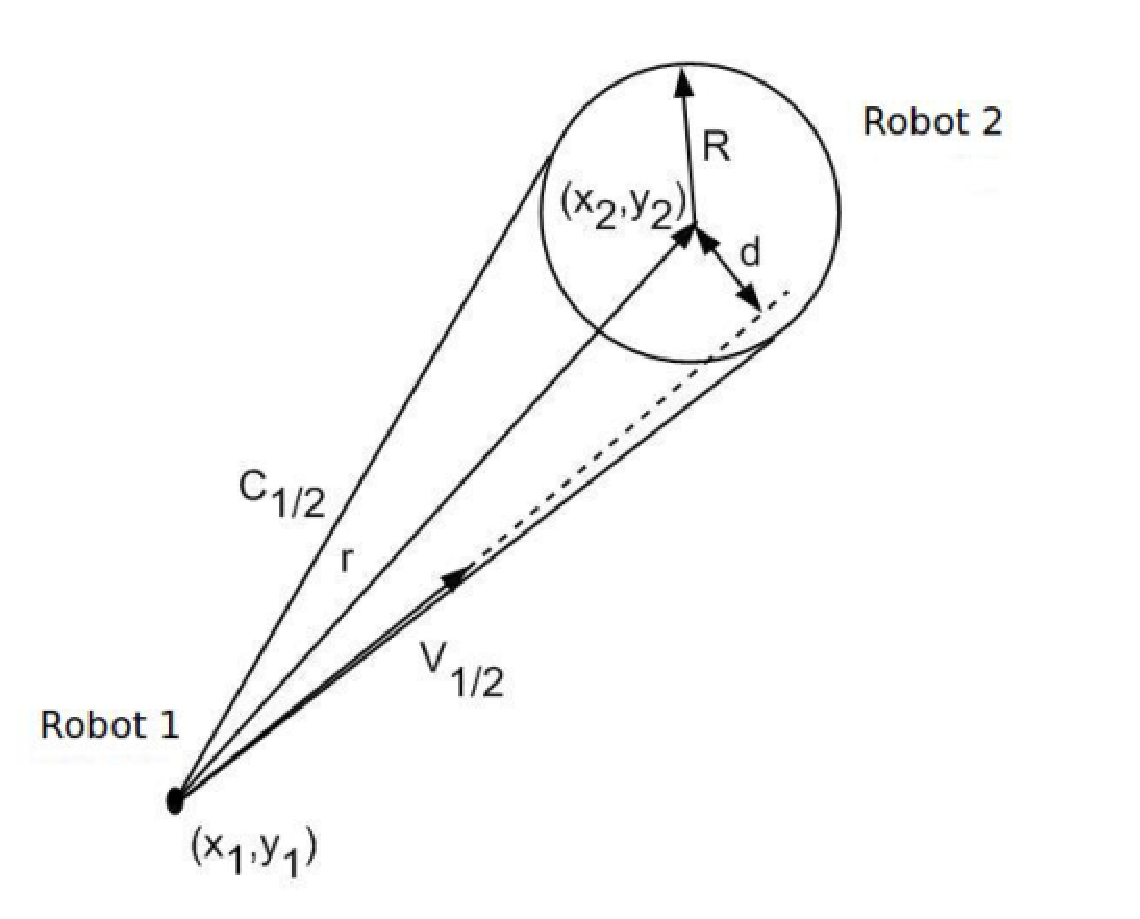
\includegraphics[width= 4.1cm, height=3.5cm]{fig3.eps}
\\
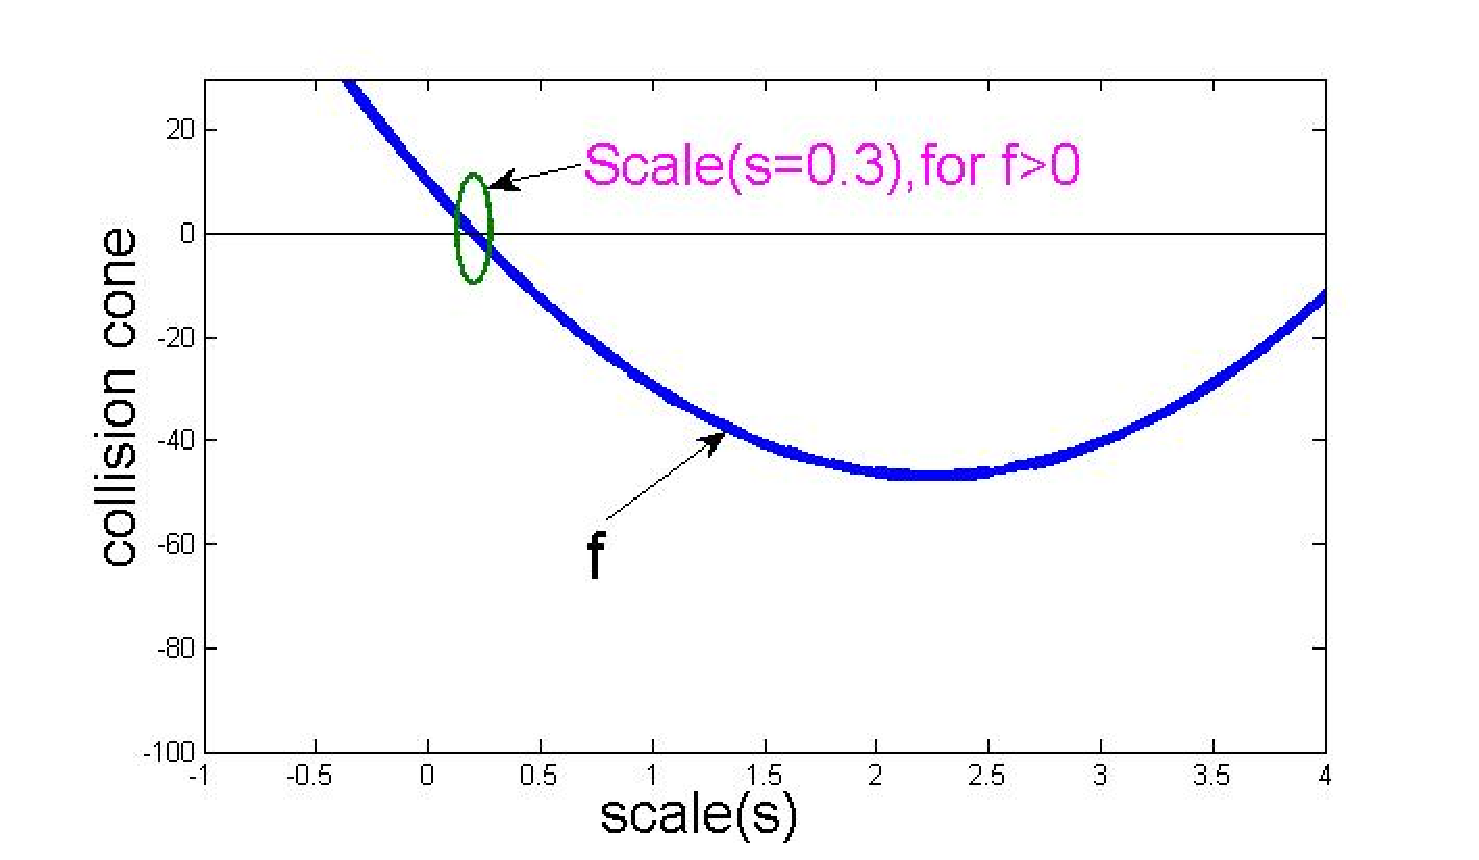
\includegraphics[width= 4.1cm, height=3.5cm]{fig4.eps}
\end{figure}
%You can also highlight sections of your presentation in a block, with it's own title

\end{frame}
\begin{frame}{Proactive collision avoidance in intent space}
\begin{block}{Probabilistic version of time scaled collision cone}
\begin{itemize}


\item{if at time $t=t_c$ the obstacles state are given by }
$$x_i^{t_c} = \mathcal{N}(\mu_i^{x},\sigma_i^{x}), \dot{x}_i^{t_c} = \mathcal{N}(\mu_i^{\dot{x}},\sigma_i^{\dot{x}})$$
$$y_i^{t_c} = \mathcal{N}(\mu_i^{y},\sigma_i^{y}), \dot{y}_i^{t_c} = \mathcal{N}(\mu_i^{\dot{y}},\sigma_i^{\dot{y}})$$
%You can also highlight sections of your presentation in a block, with it's own title
\item{Then the objective would be to find the scale that maximizes}
$$P(f_i^s \geq 0)$$ 
\end{itemize} 
\end{block}
\end{frame}
\begin{frame}{Proactive collision avoidance in intent space}
\begin{block}{Objective}

$$\underset{s}{\operatorname{argmax}}\{P(f_i^s \geq 0)\}$$ 

%You can also highlight sections of your presentation in a block, with it's own title
\end{block}
\begin{block}{Challenge}
\begin{itemize}


\item{$f_i^s is$ a random variable with unknown analytical  expression for its probability
 distribution.}
 \end{itemize} 
\end{block}
\end{frame}
\begin{frame}{Proactive collision avoidance in intent space}
\begin{figure}
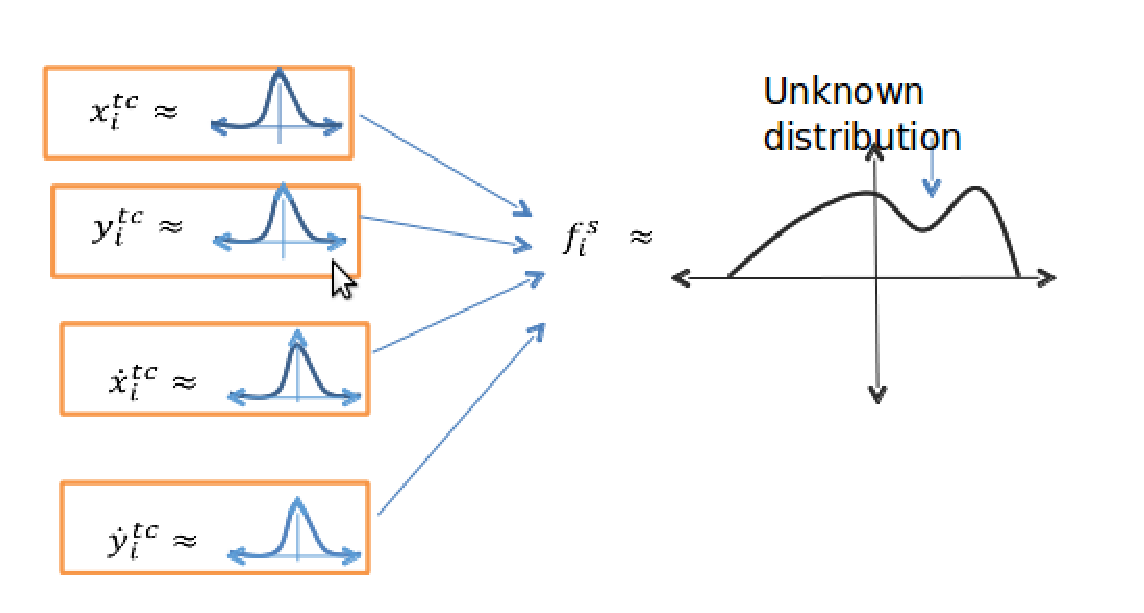
\includegraphics[width= 8.1cm, height=4.5cm]{fig8.eps}
\end{figure}
%You can also highlight sections of your presentation in a block, with it's own title

\end{frame}
\begin{frame}{Proactive collision avoidance in intent space}

%You can also highlight sections of your presentation in a block, with it's own title

\begin{block}{Solution}
\begin{itemize}


\item{Though the pdf of $f_i^s is$ does not have an analytical expression we can get its mean and standard deviation in closed form as a function of $s$}
\item{By the law of unconscious statistician}
$$E[f_i^s]=\mu_{f_i^s}=\int_{-\infty}^{\infty}\int_{-\infty}^{\infty}\int_{-\infty}^{\infty}
\int_{-\infty}^{\infty}f_i^s(.)P_i(.)dx_i^{t_c}dy_i{t_c}d\dot{x_i}^{t_c}d\dot{y_i}^{t_c}$$
\item{Which evaluates as}
$$\mu_{f_i^2} = A_is^2+B_is+C_i$$
Where $A_i,B_i$ and $C_i$ are the function of robot states and obstacle distribution parameters , $\mu_i^1,\mu_i^2,\sigma_i^1,\sigma_i^2$
 \end{itemize} 
\end{block}
\end{frame}
\begin{frame}{Proactive collision avoidance in intent space}

%You can also highlight sections of your presentation in a block, with it's own title

\begin{block}{Solution}
\begin{itemize}


\item{Similarly}
$$ \sigma_{f_i^s} = \sqrt{E[(f_i^s - E[f_i^s])^2} = 
\sqrt{D_is^4+E_i^3+F_i^2+G_is+H}$$
Where $D_i,E_i,F_i,G_i$, and $H_i$ are the function of robot states and obstacle distribution parameters , $\mu_i^1,\mu_i^2,\sigma_i^1,\sigma_i^2$
 \end{itemize} 
\end{block}
\end{frame}
\begin{frame}{Proactive collision avoidance in intent space}
\begin{block}{Solution}

$$\underset{s}{\operatorname{argmax}}\{P(f_i^s \geq 0)\} \Longrightarrow \mu_{f_i^s} \pm k * \sigma_{f_i^s} $$ 
This can be suitably achieved by suitably changing the value of $k$
%You can also highlight sections of your presentation in a block, with it's own title
\begin{figure}
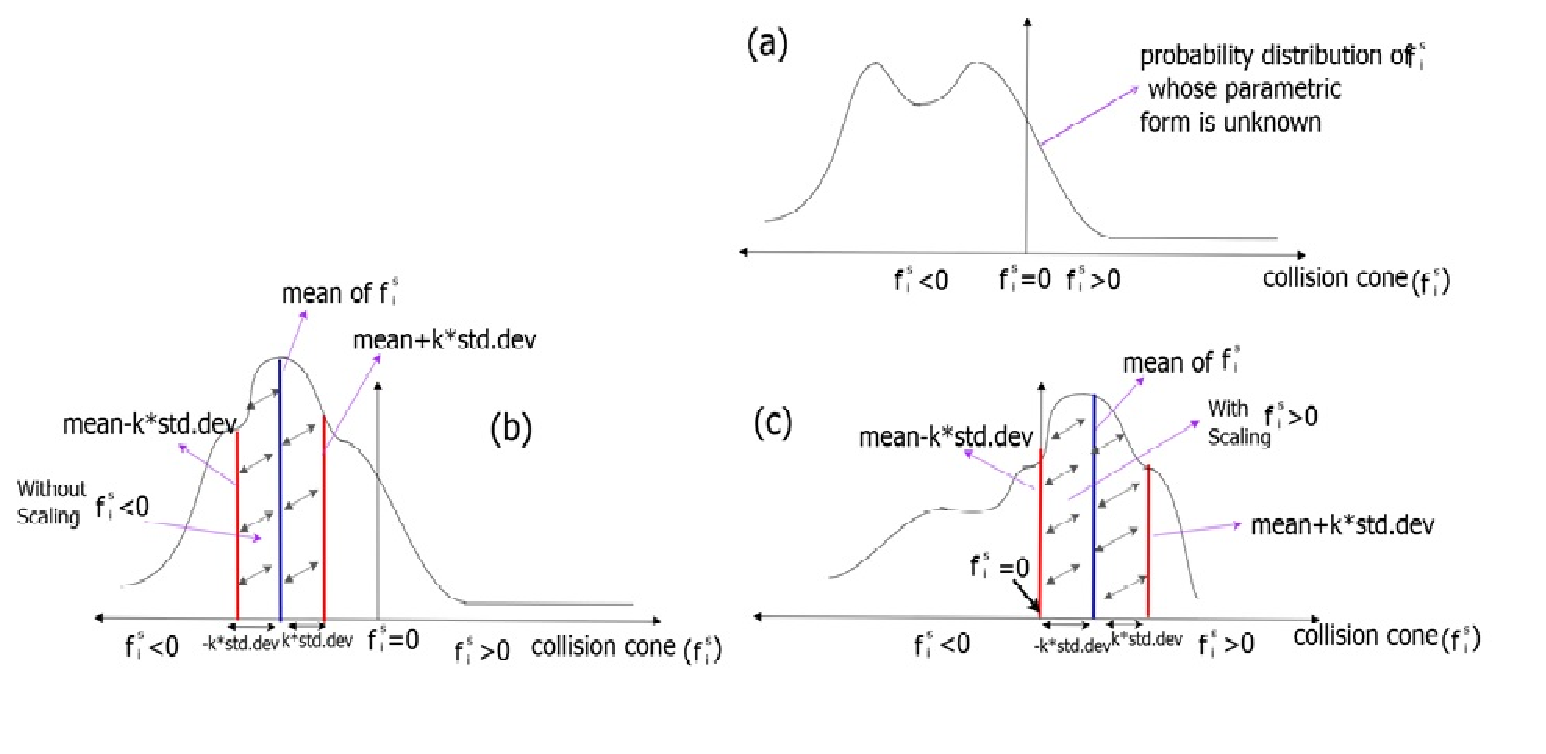
\includegraphics[width= 8.1cm, height=4.5cm]{coll_cone_distribution.eps}
\end{figure}
\end{block}
\end{frame}
begin{frame}{Proactive collision avoidance in intent space}
\begin{block}{Lower bound on $P(f_i^s) \geq 0)$}

\begin{itemize}
\item{In the previous section we found out on how to obtain scale $s$ for various values of $k$ that would end up maximizing  $P(f_i^s) \geq 0)$}
\item{Since the pdf of $P(f_i^s) \geq 0)$ does not have an analytical form ,it is not possible to get the probability of $f_i^s$ for a particular value of $s$}
\item{Hence we can only bound $P(f_i^s) \geq 0)$ by a lower bound and this can be done by Cantelli's inequality.}

\end{itemize}
\end{block}
\end{frame}
\end{block}
\end{frame}
begin{frame}{Proactive collision avoidance in intent space}
\begin{block}{Lower bound on $P(f_i^s) \geq 0)$}

\begin{itemize}
\item{The lower bound are thus obtained through}
$$ $$
\item{Thus solving for larger $k$ increases the lower bounds and thus improves the confidence measures}
\end{itemize}
\end{block}
\end{frame}
\section*{Summary}

\begin{frame}{Summary}
  \begin{itemize}
  \item
    The \alert{first main message} of your talk in one or two lines.
  \item
    The \alert{second main message} of your talk in one or two lines.
  \item
    Perhaps a \alert{third message}, but not more than that.
  \end{itemize}
  
  \begin{itemize}
  \item
    Outlook
    \begin{itemize}
    \item
      Something you haven't solved.
    \item
      Something else you haven't solved.
    \end{itemize}
  \end{itemize}
\end{frame}



% All of the following is optional and typically not needed. 
\appendix
\section<presentation>*{\appendixname}
\subsection<presentation>*{For Further Reading}

\begin{frame}[allowframebreaks]
  \frametitle<presentation>{For Further Reading}
    
  \begin{thebibliography}{10}
    
  \beamertemplatebookbibitems
  % Start with overview books.

  \bibitem{Author1990}
    A.~Author.
    \newblock {\em Handbook of Everything}.
    \newblock Some Press, 1990.
 
    
  \beamertemplatearticlebibitems
  % Followed by interesting articles. Keep the list short. 

  \bibitem{Someone2000}
    S.~Someone.
    \newblock On this and that.
    \newblock {\em Journal of This and That}, 2(1):50--100,
    2000.
  \end{thebibliography}
\end{frame}

\end{document}


